\chapter{Analysis}
\label{chap:analysis}

This chapter is dedicated to the problems that arose during the work on the project and explains the major decisions
that were made. The chapter is divided into the following sections:
\begin{itemize}
    \item \ref{general_architecture} \textbf{General Architecture} – explains the chosen suggester architecture and
    how it could be combined into the overall OpenGrok architecture.
    \item \ref{opengrok_modifications} \textbf{Opengrok Modifications} – describes the major modifications that had
    to be made in OpenGrok code to enable suggester functionality.
    \item \ref{suggester_module} \textbf{Suggester} – provides detailed explanation of how the suggester functionality
    was implemented.
\end{itemize}

\section{General Architecture}
\label{general_architecture}
One of the most important aspects of software products is their architecture. If the architecture does not take into account some
quality attributes then they are very hard to implement in the underlying code. When designing a high level architecture,
there were multiple solutions from which to choose:
\begin{itemize}
    \item \textbf{Implement suggester in the Web module} – probably the easiest solution. There would be no inter-tier
    boundaries; therefore, no need to define public API
    \footnote{\url{https://en.wikipedia.org/wiki/Application\_programming\_interface}}. Also, there would be no need
    to add any other configurations to the build scripts. However, this seems like a step towards a monolithic application
    \footnote{\url{https://en.wikipedia.org/wiki/Monolithic\_application}} which has proven to be harder to maintain in the
    long run.
    \item \textbf{Implement suggester as a separate module} – suggester could be implemented as an additional module to
    the already modular architecture described in \ref{opengrok_modules}. This new module could be a dependency of the Web
    module which would need to be modified to parse and process the data that are passed in. These data then could be
    passed to the new module via its public API. The result would look like shown in the Figure \ref{opengrok_modules_changed_img}.
    \begin{figure}[htbp]
    \centering
    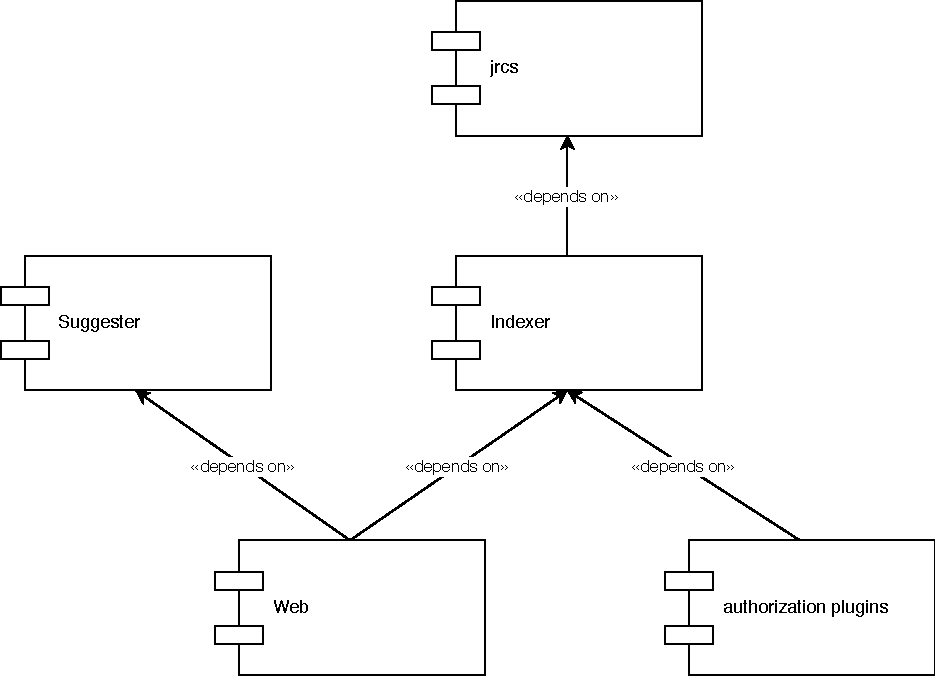
\includegraphics[width=100mm]{../img/opengrok_modules_changed.pdf}
    \caption{OpenGrok modules with Suggester module}
    \label{opengrok_modules_changed_img}
    \end{figure}
    \item \textbf{Implement suggester as a separate service} – this is a step towards microservices architecture
    \footnote{\url{https://en.wikipedia.org/wiki/Microservices}}. The suggester would run as a separate program
    listening on a different port and possibly on a different machine. Therefore; the implementation could be in any
    programming language and not necessarily in Java. Also, this could enable easy scalability of this service,
    e.g. one service per project. However, the suggester would still require access to the index files.
\end{itemize}

\textbf{Chosen solution} – in the end, the second proposal was chosen. Implementing suggester as a separate module is a
good compromise between a separate service and implementing it in the Web module. The main reason for this choice was that
OpenGrok does not support installation or scalability across multiple machines and these features are not planned to be
implemented in the near future. Therefore, it could be hard for users to set up and configure this new service.
However, the suggester module needs to have a public API and does not depend on any other OpenGrok modules. Therefore, it
will not require a lot of changes to bundle it as a separate service if the need arises in the future.

\section{OpenGrok Modifications}
\label{opengrok_modifications}

As discussed in \ref{general_architecture}, the Suggester is added as a separate module which is a dependency of the
OpenGrok Web module. Therefore, changes to the Web module are required. OpenGrok uses the Maven module structure.
Thus, the Suggester module has to respect it as well.

\subsection{Frontend}

As described in \ref{opengrok-web} section, OpenGrok provides a web interface. Some parts of the web need to be modified
for the Suggester support.

\subsubsection{Configuring Suggester}
OpenGrok provides REST API endpoint for querying or manipulating the configuration of the Web application.
This endpoint could be used to retrieve the suggester configuration and apply it.
However, this endpoint is only reachable from the targeted machine because of security reasons.
Therefore, it is needed to bypass this limitation and provide one endpoint which will return only the suggester configuration.
This endpoint could also filter the information which is redundant to the JavaScript implementation.

\subsubsection{Showing the Suggestions}
\label{showing_suggestions}

The Suggester needs to detect if the user pressed a key while having a specific input selected for which it is enabled. Upon
detecting this change, it needs to process the data, send it to the backend part of the software, processs the returned
result and show it to
the user. All this should be as quick as possible so the user considers it to be seamless.

In the field of search engines, speed is very important. According to \citep{marissa_mayers},
Marissa Mayer\footnote{\url{https://en.wikipedia.org/wiki/Marissa\_Mayer}}, former
Yahoo!\footnote{\url{https://en.wikipedia.org/wiki/Yahoo!}}
CEO\footnote{\url{https://en.wikipedia.org/wiki/Chief_executive_officer}}, spoke at the
2006 Web 2.0 conference where she said that $0.5s$ drop in speed reduced the traffic by $20\%$.

Showing suggestions is considered to be a response to control activation. This is an indication that some control member
(in our case keyboard key) has been physically activated. Based on \citep{response_time}, the response
should take no more than $100ms$ in order for the system to be considered unobtrusive.

Simplified picture of the
steps that need to be taken is shown in the Figure \ref{suggest_sequence}.

\begin{figure}[htbp]
\centering
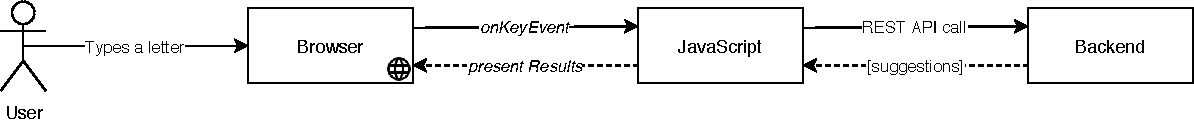
\includegraphics[width=145mm]{../img/opengrok_sequence.pdf}
\caption{Typical suggestions workflow}
\label{suggest_sequence}
\end{figure}

There are many libraries which provide "JavaScript" functionality as shown in Figure \ref{suggest_sequence},
the most notable are:
\begin{itemize}
    \item jQuery UI Autocomplete\footnote{\url{https://jqueryui.com/autocomplete/}}
    \item Ajax Autocomplete for jQuery\footnote{\url{https://www.devbridge.com/sourcery/components/jquery-autocomplete/}}
    \item MagicSuggest\footnote{\url{http://nicolasbize.com/magicsuggest/}}
\end{itemize}

All of the above require jQuery\footnote{\url{http://jquery.com}} library which is already included in the OpenGrok.
In the end, jQuery UI Autocomplete was chosen because jQuery UI was already used by OpenGrok. Although, the Autocomplete
module was not included. jQuery UI Autocomplete provides an easy-to-use API and is easily customizable; these factors
also contributed to the decision of picking this library.

\paragraph{Data format}
As mentioned, user's input must be sent to the backend part of the software, processed and
returned back. jQuery UI Autocomplete supports the JSON\footnote{\url{https://www.json.org}} format by default. This format
is widely used and performs better than XML in this
specific situation (\url{https://www.w3schools.com/js/js_json_xml.asp}). Also OpenGrok's REST API supports
automatic conversion to JSON objects via the Jackson\footnote{\url{https://github.com/FasterXML/jackson}} library.
Therefore, it is a solid choice.

\subsubsection{Detecting the Token for Suggestions}
As referenced in \ref{opengrok_usage}, it is possible to write multiple tokens into one \textit{input} HTML tag.
Imagine the text: "car engine". With only this information the Suggester is not able to tell if it should show
suggestions for the "car" prefix or "engine" prefix or something totally different. Therefore, the Suggester also requires the position of the last typed
key.

The position needs to be retrieved and set by the JavaScript part of the web page. This functionality could be written in
pure JavaScript; however, simple, small, and easy-to-use library \textit{jQuery caret} (\url{https://github.com/acdvorak/jquery.caret})
was used instead.

\subsection{Backend}
As stated in \ref{showing_suggestions}, the server part needs to have a service which returns results based on the
input typed by the user. And as mentioned in \ref{opengrok-web}, the Web module is a web application compliant with
the servlet API; therefore, a new servlet which listens to the user's input and returns suggestions needs to be added.

\subsubsection{How to Implement the Suggester Servlet}
The servlet represents a simple REST API endpoint
because it needs to respond to HTTP GET requests and return the response in JSON.
There is a lot of options how this could be achieved; however, the most notable are:
\begin{itemize}
    \item Use default implementation by extending \textit{HttpServletRequest} and its method \textit{doGet()}. The main
    advantage of this approach is that there are no other dependencies because they are provided by the underlying servlet container.
     However, some boilerplate code would need
    to be written which could be avoided.
    \item Use JAX-RS API and its implementation Jersey\footnote{\url{https://jersey.github.io}}. With this approach the
    code can be clean and much easier to understand because of the use of provided annotations from JAX-RS API.
    Not to mention that Jersey provides additional features:
    \begin{itemize}
        \item Dependency injection.
        \item Bean validation support.
        \item Automatic JSON conversion using Jackson library.
    \end{itemize}
\end{itemize}

Since OpenGrok Web has already REST API support and both JAX-RS API and Jersey already on the classpath,
there is no dependency overhead. As a result, the second option was chosen.

\subsubsection{Processing User Input}
\label{processing_user_input}
As referenced in \ref{opengrok_usage}, OpenGrok web interface provides multiple HTML \textit{input} fields which
represent different Lucene \textit{fields} which should be searched. Each of these input fields can contain some value.
Therefore, all these values are passed to the server along with the information of the currently selected input field and
the caret position in it.

Each of these fields can include any form of Lucene query, as stated in \ref{opengrok_usage}. Since these queries might
get very complicated, a proper parser is needed. Exactly for this purpose, OpenGrok provides modified parsers from Lucene library.


The character position is
useless after the parsing is done – it is not possible to find the token it referenced anymore. Therefore, a small
trick can be used. Before parsing the text data, a short, random but regarding the text unique string of characters
is generated and inserted at the mentioned position. From now on, it is possible to use just this identifier since it
uniquely identifies the token in which the user is currently interested. However, this presents also a small disadvantage.
If the query typed by the user is not correct, then Lucene parser generates \textit{ParseException} which contains
this identifier; therefore, it might be a little harder to decode the original query from the exception's message.

\subsubsection{Reacting to the Events}

Running OpenGrok Web instance has REST API which allows the Indexer or administrators to indicate that some event occurred.
More information can be found in \ref{opengrok_rest}. Events that the Suggester should be able to react to:
\begin{itemize}
    \item \textbf{Configuration change} – \textit{PUT /api/v1/configuration}

    Suggester should rebuild to be in concordance with the new configuration.
    \item \textbf{Indication to refresh index searchers} – \textit{PUT /api/v1/system/refresh}

    Most of the time this message indicates that the reindex of the data has been done. The Suggester
    should update its data to be up to date.

    \item \textbf{Marking project as indexed} – \textit{PUT /api/v1/projects/{project}/indexed}

    OpenGrok can be aware of projects which are not yet indexed. It is not possible to search in these projects;
    as a result, there is no need for suggester to know about them. However, this changes if the project is marked as indexed.
    The Suggester should then build its inner data to support suggestions for the project.

    \item \textbf{Project delete} – \textit{DELETE /api/v1/projects/{project}}

    Suggester should drop any data it has regarding the project.
\end{itemize}

\section{Suggester}
\label{suggester_module}
This section looks at the Suggester module in more detail. First of all, it describes all the queries the suggester supports.
Then, it looks at the fuzzy and boost factors. After that, it discusses how to leverage the previous searches. At last, it mentions some
additional properties that were needed by this module.

\subsection{Prefix Query}
\label{prefix_query}
To start with, let's look at the simplest and at the same time probably the most used case. \textbf{Prefix query} is a special case of
\textit{Wildcard query} \ref{wildcard_query}.
It can be divided into 2 parts:
\begin{itemize}
    \item \textbf{prefix} – text which represents the prefix of all the terms this query accepts.
    \item \textbf{*} – wildcard symbol which accepts any text (even zero-length text).
\end{itemize}

These parts are then combined together as: \textit{\{prefix\}*}.
It is probably the most used case because of the suggester's nature. If the user types any simple text (even without \textit{*}) then
the suggester automatically appends \textit{*} to the end and considers this as a prefix query to provide adequate suggestions.

Since the prefix queries will be used that often then the suggester needs to be optimized for this type of queries.

\subsubsection{Scoring}
\label{prefix_scoring}
Every term needs to have a \textit{score} associated with it so the suggester can decide which term is better suited
to appear as a suggestion. Therefore, the problem is not only to find the terms with a specific prefix but to find $n$
terms with the best scores having the specific prefix. Let's assume that the suggester does not have any information
about the previous searches. This case is discussed in
\ref{previous_searches}. The suggester has access to the Lucene index provided by the Indexer. % TODO: add refs?
Therefore; it has access to:
\begin{itemize}
    \item \textbf{Total term frequency $T$} – how many times the term appears in the document set.
    \item \textbf{Document frequency $N$} – in how many documents does the term appear.
    \item \textbf{Number of documents $D$} – total number of documents in the document set.
\end{itemize}

\paragraph{IDF\protect\footnote{\url{https://en.wikipedia.org/wiki/Tf\%E2\%80\%93idf\%23Inverse\_document\_frequency\_2}}}
At a first glance, it might seem as a good idea to use inverse document frequency as a metric. The formula for computing this metric can be seen at \ref{IDF_eq}.
\begin{equation}
\label{IDF_eq}
IDF(t) = \log{\frac{D}{N}}
\end{equation}
Basically, it says how important the term is in the document set. If the term occurrs in every document, then it is probably
a very common word. If provided in the query, it does not reduce the size of the result set significantly.
However, this importance is correct if the term is
provided by the user in the query. If the suggester were to use it, then it would suggest terms that are used the least, e.g. only once.
Therefore; this is not a good scoring option.

\paragraph{Document frequency}
Document frequency is a good indicator of how the term is used throughout the document set. However,
this metric is specific to the project. Thus, it would be hard to compare values across multiple projects. The solution
to the problem is normalization. Resultant equation can be seen at \ref{norm_doc_freq}.
\begin{equation}
\label{norm_doc_freq}
score = \frac{N}{D} \cdot constant
\end{equation}
This metric gives results which are expected of the suggester; therefore, it is the best option so far.

% TODO: find some work on this?

\subsubsection{Possible Implementations}
\label{possible_implementations}
As mentioned before, the implementation should be fast to be able to fulfill the users' expectations. Although, at the
same time, it should not waste memory resources. One data structure per Lucene field per project is needed. The OpenGrok
installation can contain hundreds of projects and depending on the size of the project, one Lucene field can possibly contain
tens of thousands of terms or even more (in some cases millions).

\paragraph{Trie\protect\footnote{\url{https://en.wikipedia.org/wiki/Trie}}} – sometimes called prefix tree, is the simplest
structure suitable for our purposes. However, it does not support efficient lookup based on scores. It would
be needed to traverse the whole subtree for a specific prefix to find the terms with the best scores.

\paragraph{Ternary search tree\protect\footnote{\url{https://en.wikipedia.org/wiki/Ternary\_search\_tree}}} – is a
special case of Trie. Same as Trie, it does not have any support for more efficient lookup based on scores.

\paragraph{FST\protect\footnote{\url{https://en.wikipedia.org/wiki/Finite-state\_transducer}}} \label{FST} – is a finite state
automaton which can produce output. Special case of FST is a weighted FST (WFST) where each transition can have an
associated weight. It is possible to construct a WFST which will provide a very efficient algorithm for finding the
$n$ terms with the best scores. This algorithm is explained in \citep{Mohri02anefficient}. However, this algorithm returns
terms with the lowest scores and based on the chosen scoring it is needed for it to return the terms with the highest
scores. This can be achieved by a neat trick; it is possible to invert the score by the formula \ref{invert_score}.
\begin{equation}
\label{invert_score}
newScore = maxPossibleScoreValue - score
\end{equation}
An efficient construction of minimal, acyclic and deterministic WFST is explained in \citep{Mihov01directconstruction}.

\textbf{Example} – WFST with terms and weights: $CAR = 10, CARS = 15, CART = 5$ can be seen in \ref{wfst_example}.

\begin{figure}[htbp]
\centering
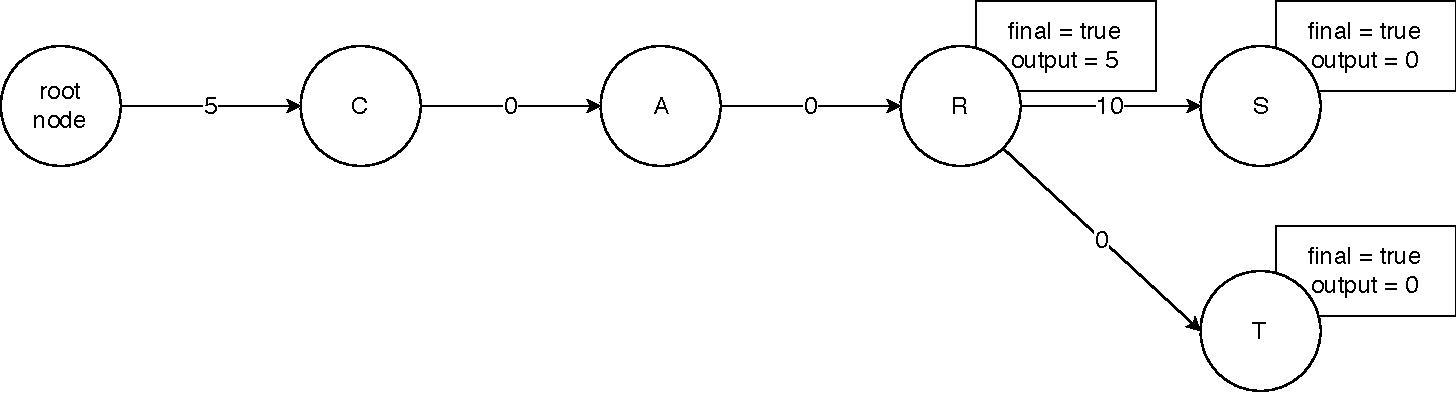
\includegraphics[width=145mm]{../img/wfst.pdf}
\caption{WFST example}
\label{wfst_example}
\end{figure}

% TODO: describe algorithm?

\paragraph{Comparison}

Two datasets were used:
\begin{itemize}
    \item \textbf{English words} – list of \textbf{370,099} words freely available at \url{https://github.com/dwyl/english-words}.
    \item \textbf{Linux kernel} – \textit{full} field of indexed Linux kernel with \textbf{3,459,733} terms.
\end{itemize}

% TODO: useful info average term length in Linux kernel: 22.033919380483987

Measured was the average time of specific operations on the data structures.
The description of the test cases:
\begin{itemize}
    \item \textbf{"non" Prefix Lookup} – is a lookup of 10 words with the prefix "non" which is the most occurring prefix
    of length 3 in the English words dataset with 7479 occurrences. Linux kernel has only 644 occurrences. Results can be seen
    on the graph \ref{comp_non}.

    \begin{figure}[htbp]
        \centering
        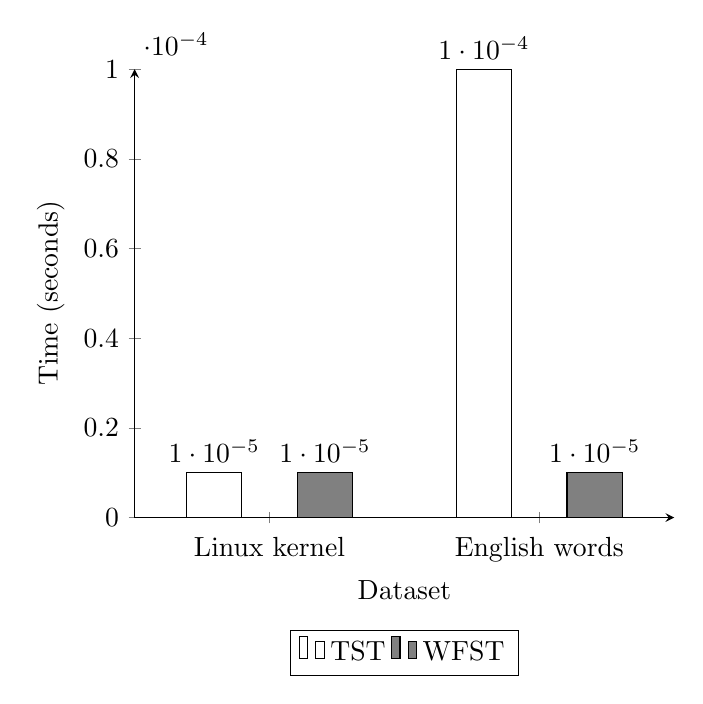
\begin{tikzpicture}
            \begin{axis}[
                ybar=20pt,
                bar width=20pt,
                xlabel={Dataset},
                ylabel={Time (seconds)},
                ymin=0,
                xtick=data,
                axis x line=bottom,
                axis y line=left,
                enlarge x limits=0.5,
                symbolic x coords={Linux kernel, English words},
                xticklabel style={anchor=base,yshift=-\baselineskip},
                nodes near coords={\pgfmathprintnumber\pgfplotspointmeta},
                legend style={at={(0.5,-0.25)},anchor=north,legend columns=-1}
            ]
            \addplot[ybar, fill=white, error bars/.cd, y dir=both, y explicit] plot coordinates {
            (English words, 0.0001)
            (Linux kernel, 0.00001)
            };

            \addplot[ybar, fill=gray, error bars/.cd, y dir=both, y explicit] plot coordinates {
            (English words, 0.00001)
            (Linux kernel, 0.00001)
            };
            \legend{TST, WFST}
            \end{axis}
        \end{tikzpicture}
        \caption{"non" Prefix Lookup comparison}
        \label{comp_non}
    \end{figure}
    \item \textbf{One Letter Prefix Lookup} – is a lookup of 10 words with the prefix of each letter from the basic alphabet.
    Results can be seen the on the graph \ref{comp_one}.

    \begin{figure}[htbp]
        \centering
        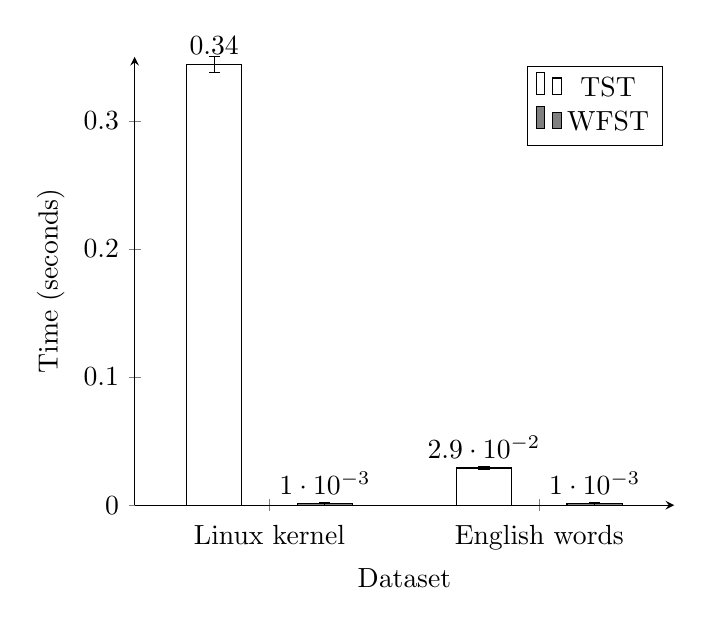
\begin{tikzpicture}
            \begin{axis}[
                ybar=20pt,
                bar width=20pt,
                xlabel={Dataset},
                ylabel={Time (seconds)},
                ymin=0,
                xtick=data,
                axis x line=bottom,
                axis y line=left,
                enlarge x limits=0.5,
                symbolic x coords={Linux kernel, English words},
                xticklabel style={anchor=base,yshift=-\baselineskip},
                nodes near coords={\pgfmathprintnumber\pgfplotspointmeta}
            ]
            \addplot[ybar, fill=white, error bars/.cd, y dir=both, y explicit] plot coordinates {
            (English words, 0.029) += (English words, 0.001) -= (English words, 0.001)
            (Linux kernel, 0.344) += (Linux kernel, 0.006) -= (Linux kernel, 0.006)
            };

            \addplot[ybar, fill=gray, error bars/.cd, y dir=both, y explicit] plot coordinates {
            (English words, 0.001) += (English words, 0.001) -= (English words, 0.001)
            (Linux kernel, 0.001) += (Linux kernel, 0.001) -= (Linux kernel, 0.001)
            };
            \legend{TST, WFST}
            \end{axis}
        \end{tikzpicture}
        \caption{One Letter Prefix Lookup comparison}
        \label{comp_one}
    \end{figure}

    \item \textbf{Two Letter Prefix Lookup} – is a lookup of 10 words with the prefix which is a combination of 2 letters
    from the basic alphabet. Results can be seen on the graph \ref{comp_two}.

    \begin{figure}[htbp]
        \centering
        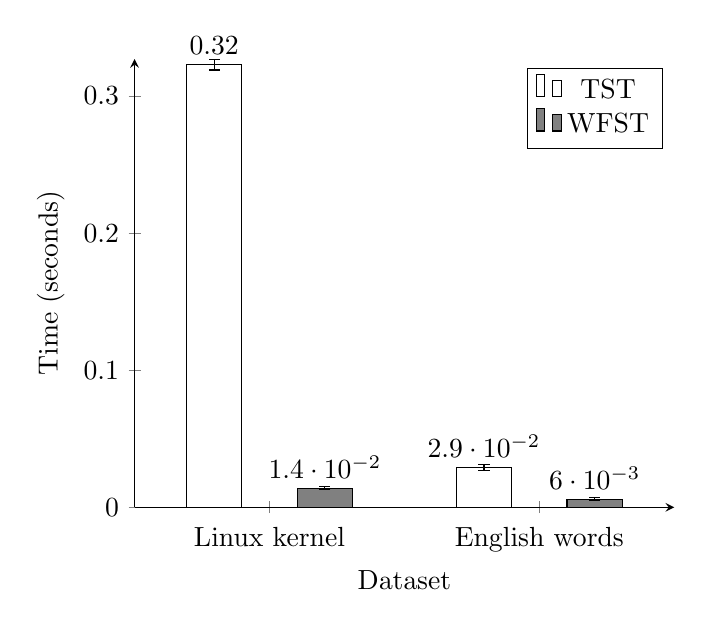
\begin{tikzpicture}
            \begin{axis}[
                ybar=20pt,
                bar width=20pt,
                xlabel={Dataset},
                ylabel={Time (seconds)},
                ymin=0,
                xtick=data,
                axis x line=bottom,
                axis y line=left,
                enlarge x limits=0.5,
                symbolic x coords={Linux kernel, English words},
                xticklabel style={anchor=base,yshift=-\baselineskip},
                nodes near coords={\pgfmathprintnumber\pgfplotspointmeta}
            ]
            \addplot[ybar, fill=white, error bars/.cd, y dir=both, y explicit] plot coordinates {
            (English words, 0.029) += (English words, 0.002) -= (English words, 0.002)
            (Linux kernel, 0.323) += (Linux kernel, 0.004) -= (Linux kernel, 0.004)
            };

            \addplot[ybar, fill=gray, error bars/.cd, y dir=both, y explicit] plot coordinates {
            (English words, 0.006) += (English words, 0.001) -= (English words, 0.001)
            (Linux kernel, 0.014) += (Linux kernel, 0.001) -= (Linux kernel, 0.001)
            };
            \legend{TST, WFST}
            \end{axis}
        \end{tikzpicture}
        \caption{Two Letter Prefix Lookup comparison}
        \label{comp_two}
    \end{figure}

    \item \textbf{Build time} – performs build of the data structure from the scratch. Results can be seen on the graph
    \ref{comp_build}.

    \begin{figure}[htbp]
        \centering
        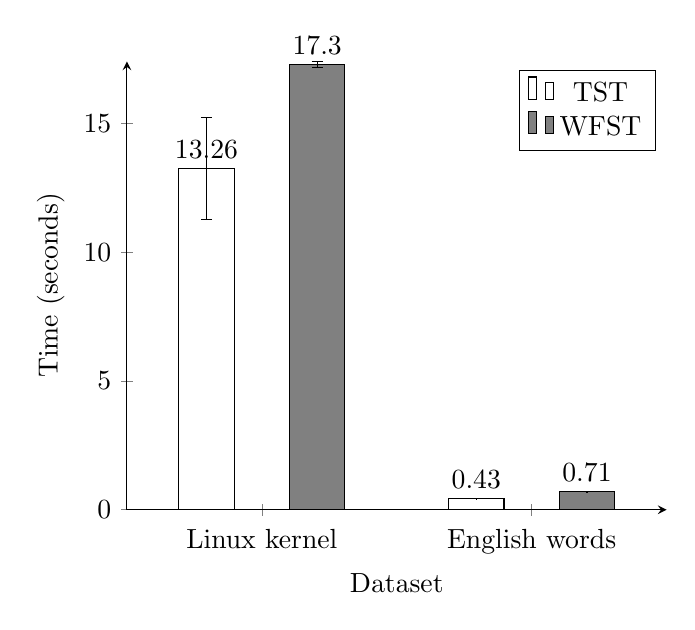
\begin{tikzpicture}
            \begin{axis}[
                ybar=20pt,
                bar width=20pt,
                xlabel={Dataset},
                ylabel={Time (seconds)},
                ymin=0,
                xtick=data,
                axis x line=bottom,
                axis y line=left,
                enlarge x limits=0.5,
                symbolic x coords={Linux kernel, English words},
                xticklabel style={anchor=base,yshift=-\baselineskip},
                nodes near coords={\pgfmathprintnumber\pgfplotspointmeta}
            ]
            \addplot[ybar, fill=white, error bars/.cd, y dir=both, y explicit] plot coordinates {
            (English words, 0.433) += (English words, 0.01) -= (English words, 0.01)
            (Linux kernel, 13.264) += (Linux kernel, 1.978) -= (Linux kernel, 1.978)
            };

            \addplot[ybar, fill=gray, error bars/.cd, y dir=both, y explicit] plot coordinates {
            (English words, 0.706) += (English words, 0.003) -= (English words, 0.003)
            (Linux kernel, 17.296) += (Linux kernel, 0.12) -= (Linux kernel, 0.12)
            };
            \legend{TST, WFST}
            \end{axis}
        \end{tikzpicture}
        \caption{Comparison of build times}
        \label{comp_build}
    \end{figure}


    \item \textbf{Memory usage} – approximate sizes the data structures use in the computer's main memory.
     The result can be seen on the graph \ref{comp_mem}. The data was measured by calling method
     \textit{ramBytesUsed()} which is a custom method commonly implemented in Lucene's data structures.
     The drastic
    difference is mainly due to WFST's implementation which was optimized to use as little memory as possible while
    providing a very solid performance. Some of the WFST' optimizations:
    \begin{itemize}
        \item Storage in byte arrays. There is no need to keep references to the objects which take 8B on 64-bit computer
        but rather smaller identifiers. Also, differences in arc weights are mostly very small. The implementation
        leverages this and encodes integers with variable length into the mentioned byte arrays.
        \item Caching of the first arcs of the FST.
        \item Constant arc size for the arcs into certain depth which allows binary search among the arcs. (Random
        access is not possible because it would require more memory which would not be used.)
    \end{itemize}
    It can be noted that some of these optimizations may hinder the performance. However, the results show that the WFST
    performs well and is memory usage efficient.

    \begin{figure}[htbp]
        \centering
        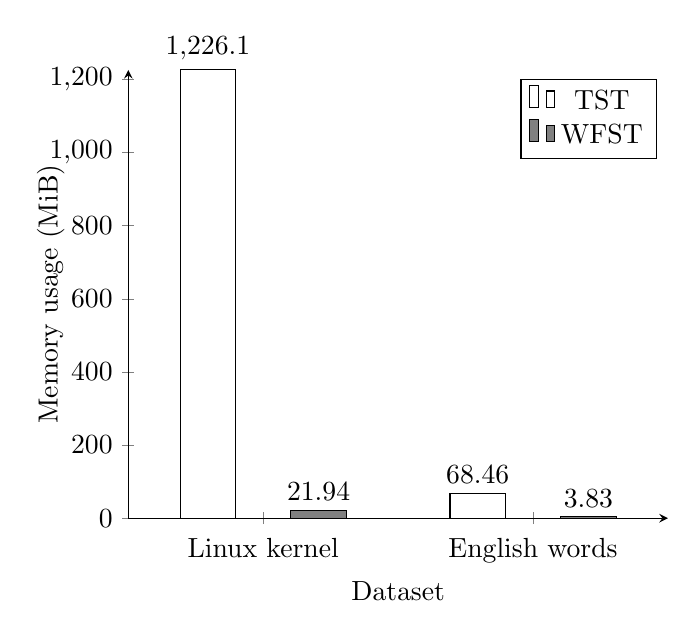
\begin{tikzpicture}
            \begin{axis}[
                ybar=20pt,
                bar width=20pt,
                xlabel={Dataset},
                ylabel={Memory usage (MiB)},
                y label style={at={(axis description cs:-0.1,.5)}},
                ymin=0,
                xtick=data,
                axis x line=bottom,
                axis y line=left,
                enlarge x limits=0.5,
                symbolic x coords={Linux kernel, English words},
                xticklabel style={anchor=base,yshift=-\baselineskip},
                nodes near coords={\pgfmathprintnumber\pgfplotspointmeta}
            ]
            \addplot[ybar, fill=white, error bars/.cd, y dir=both, y explicit] plot coordinates {
            (English words, 68.4622154236)
            (Linux kernel, 1226.1035423279)
            };

            \addplot[ybar, fill=gray, error bars/.cd, y dir=both, y explicit] plot coordinates {
            (English words, 3.8268890381)
            (Linux kernel, 21.9446716309)
            };
            \legend{TST, WFST}
            \end{axis}
        \end{tikzpicture}
        \caption{Comparison of memory usage}
        \label{comp_mem}
    \end{figure}

\end{itemize}

How to reproduce these benchmarks and description of the machine on which they were run can be found in \ref{benchmark_attachment}.

Based on the provided results, it can be noted that WFST performs much better at lookups. Mainly at lookups with a short prefix.
Also, the memory usage is inarguably better in the WFST data structures. However, its build time is worse by a small margin than TST's.

OpenGrok installation can easily contain dozens of projects, each of these projects contains 5 Lucene fields
(full, defs, refs, path, hist) which needs to have a suggester support. Depending on the size of the projects,
TST implementation could take many GiBs of the memory which is not feasible.

To conclude, WFST is a better option in almost every aspect except the build time which is not that important because of
the possibility of saving the data structures on the disk; and therefore, avoid it almost every time except when the index changes.

\subsection{Wildcard Query}
\label{wildcard_query}
The specific case of \textit{prefix*} is covered in the previous section \ref{prefix_query}. Therefore,
all the other cases of wildcard queries will be covered in this section.
The implementation of WFST cannot be used because of its nature.
There is no way to efficiently search in WFST tokens for the query of type \textit{*sufffix}. The required result is
the same as for the prefix query: to find the terms which are accepted by the query with the top score. However, the data
structure which could achieve this for generic wildcard query with the WFST performance is not known to the author.
Nonetheless, the Lucene evaluation of wildcard queries could be leveraged. An automaton specific to the wildcard query is
created and then the terms are filtered using this automaton. The implemenation is slower than WFST because all the terms
need to be filtered once if they are accepted by the automaton then they need to be filtered for the second time based on
their score.

\subsubsection{Scoring}
Scoring used is the same as mentioned in \ref{prefix_scoring}.

\subsection{Regular Expression Query}
The regular expression queries can be implemented in the same way as wildcard queries \ref{wildcard_query}. The only difference
is that the automaton is created based on the regular expression rules.

\subsection{Phrase Query}
\label{suggest_phrase_query}
Phrase query is a query which specifies a collection of tokens which must occur in the documents in the specified order.
The tokens must be surrounded by double quotes, e.g. \textit{"token1 token2"}. In this example, this means that \textit{token1} must be immediately followed by
\textit{token2} in the document for it to be accepted.

\subsubsection{Evaluation}
\label{prefix_evaluation}
As mentioned in \ref{indexer:index},
Lucene stores data in the reverse document index. However, to be able to determine if one token is immediately followed by another
token, their position needs to be stored and accessed. Lucene can be configured to store this information as well.
It can easily be determined if Lucene stored this data by checking if Lucene index contains a file with a \textit{.pos}
suffix.

Evaluation of the query is straightforward. Lucene performs lookup for each token in the phrase query and intersects the
results which provides all the documents which contain all of these tokens. Then it checks if the tokens are indeed
next to each other and on correct positions.

\subsubsection{Getting the Suggestions}
\paragraph{Using shingles}
Shingle\footnote{\url{https://en.wikipedia.org/wiki/W-shingling}} is an n-gram of words. It would be possible to create
shingles of specific count (e.g. 2 to 5 words) during the indexing phase. Each shingle would be treated as a single term.
Then, it would be possible to do quick prefix lookup as described in \ref{prefix_query}. However, this solution has many drawbacks:
\begin{itemize}
    \item Another, not quite small index would have to be created.
    \item The suggestions would work for only the last token of the phrase query.
    \item The maximum number of tokens in phrase query for which the suggestions would work would be limited by the longest
    shingle.
    \item Another data structure which would contain all of the shingles for quick lookup would have to be stored in the
    main memory.
\end{itemize}

\paragraph{Using the default evaluation}
As explained in \ref{processing_user_input}, it is known which token should be considered as prefix. Therefore, this token
can be omitted but the requested position of other tokens must stay unchanged. Then the same evaluation as mentioned in
\ref{prefix_evaluation} can be used. The result of the evaluation is a pair:
\begin{itemize}
    \item Document identifier.
    \item Token position.
\end{itemize}
Based on this information it should be possible the gather all the possible terms and accept only those with the
provided prefix.

\paragraph{Getting the token at specific position}
Based on the document identifier and token position it should be easy to get the needed term. However, Lucene does not
provide any functionality to do this efficiently because the nature of the reverse document index is a complete
opposite to the data structure which would provide efficient implementation of this operation. Possible solutions are:
\begin{itemize}
    \item Implement data structure which would efficiently lookup a term based on a position and document identifier.
    However, the size of the data structure would not be trivial in comparison with the actual index size. Furthermore,
    it would slow down the indexing phase even more which might already take a few hours or even days if the projects
    being indexed are very huge.
    \item Read and tokenize the document with the specified identifier. Nonetheless, this might be a slow operation if there
    were a lot of documents accepted by the query because of the necessary
    I/O\footnote{\url{https://en.wikipedia.org/wiki/Input/output}} operations.
    \item Use the already existing reverse document index. It is possible to lookup all the terms based on the prefix.
    Then filter the terms which do not occur in the documents which were found by the phrase query and those which
    do not have the correct position in the document.
\end{itemize}

The first option is not feasible because of the added size to the already existing index. Comparison between the
second and the third option can be seen on the graph \ref{comp_phrase}.

\begin{figure}[htbp]
    \centering
    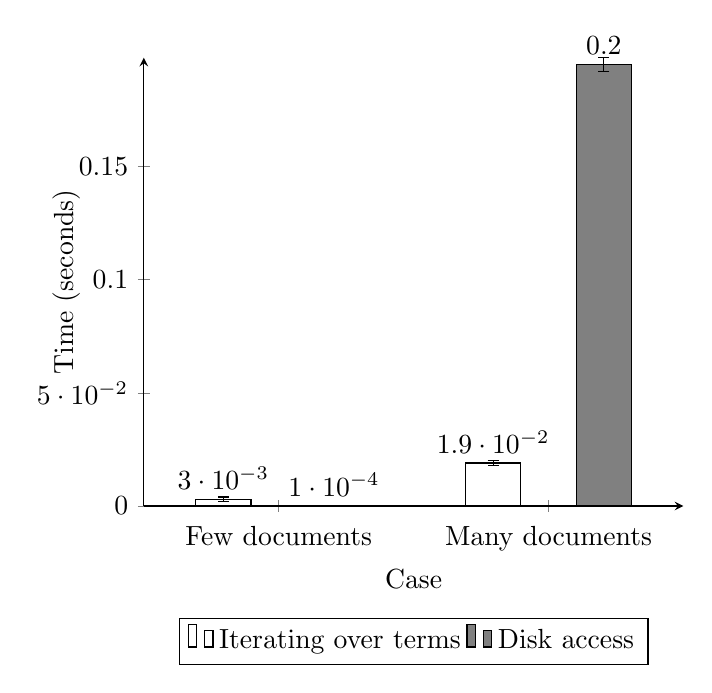
\begin{tikzpicture}
        \begin{axis}[
            ybar=20pt,
            bar width=20pt,
            xlabel={Case},
            ylabel={Time (seconds)},
            y label style={at={(axis description cs:-0.1,.5)}},
            ymin=0,
            xtick=data,
            axis x line=bottom,
            axis y line=left,
            enlarge x limits=0.5,
            symbolic x coords={Few documents, Many documents},
            xticklabel style={anchor=base,yshift=-\baselineskip},
            nodes near coords={\pgfmathprintnumber\pgfplotspointmeta},
            legend style={at={(0.5,-0.25)},anchor=north,legend columns=-1}
        ]
        \addplot[ybar, fill=white, error bars/.cd, y dir=both, y explicit] plot coordinates {
        (Few documents, 0.003) += (Few documents, 0.001) -= (Few documents, 0.001)
        (Many documents, 0.019) += (Many documents, 0.001) -= (Many documents, 0.001)
        };

        \addplot[ybar, fill=gray, error bars/.cd, y dir=both, y explicit] plot coordinates {
        (Few documents, 0.0001)
        (Many documents, 0.195) += (Many documents, 0.003) -= (Many documents, 0.003)
        };
        \legend{Iterating over terms, Disk access}
        \end{axis}
    \end{tikzpicture}
    \caption{Comparison between iterating over terms and disk access for getting the term at a specific position in document}
    \label{comp_phrase}
\end{figure}

\textit{Few documents} query matched only 2 documents whereas \textit{Many documents} query matched 738 documents.
The number of terms was 24355. For details about how the measurement was performed consult the Attachment
\ref{benchmark_attachment}.
It can be noted that for a small number of matched documents the second option is
faster than the third option. However, this changes when the number of matched documents is large. Nevertheless,
the second option has a few additional drawbacks:
\begin{itemize}
    \item It needs access to OpenGrok's Indexer module to be able to tokenize the files.
    \item There might be problems if the source code is out of sync with the index. This happens when the project source code
    is updated (e.g. \textit{git pull}) and Indexer is performing reindex.
\end{itemize}

Due to these drawbacks, the implementation where the data would be gathered by reading and tokenizing the documents was not
implemented despite the increased performance for a small number of documents. It might be considered as a possible
extension.

\subsubsection{Scoring}
It would be possible to use the same scoring as in \ref{prefix_scoring}. However, the scoring is not specific enough.
For instance, the term could have a big document frequency but in the context of phrase query would occur only once,
whereas, the term with lower document frequency could occur more times, which would make it more specific. Therefore,
the scoring based on the term frequency in the context of phrase query provides better results.

\subsection{Range Queries}
Range queries have many similarities with wildcard queries \ref{wildcard_query} in terms of implementation for the
suggester. The main difference is in creation of the automaton. Range query contains a lower and upper term. The
suggestions depends on which of the terms is used as a prefix.

\subsubsection{Lower Term as a Prefix}
First of all, the automaton $A_{int}$ which represents a binary interval is created between the lower and upper term. Then,
the automaton $A_{prefix}$ which accepts all terms with prefix specified in the lower bound is needed. The result automaton is the
intersection of these two, as in \ref{lt_automaton}.

\begin{equation}
\label{lt_automaton}
A_{result} = A_{int} \cap A_{prefix}
\end{equation}

\subsubsection{Upper Term as a Prefix}
Similarly, the automaton $A_{prefix}$ which accepts all terms with prefix specified in the upper bound is created. Then,
another binary interval automaton $A_{int}$ is needed; however, this one has no lower bound specified and for the upper bound the
lower term of the query is used. The result automaton needs to be created as a difference between the prefix automaton
and the binary interval automaton, as in \ref{ut_automaton}.

\begin{equation}
\label{ut_automaton}
A_{result} = A_{prefix} - A_{int}
\end{equation}

\subsection{Including Boolean Operators}
\label{boolean_ops}

% TODO: probably move this to OpenGrok chapter, this chapter should be about suggester

There are multiple boolean operators which can modify the meaning of the term in the query.

\subsubsection{Unary Boolean Operators}
Following unary operators are supported:
\begin{itemize}
    \item \textbf{+} unary operator in front of the term means that the term must occur in the result document set.
    \item \textbf{-} unary operator in front of the term means that the term cannot occur in the result document set.
    It is also possible to use synonyms \textbf{NOT} or \textbf{!}. However, it is not possible to use it in a query
    with a single term.
    \item \textbf{Default} unary operator – no unary operator in front of the term means that the term should occur
    in the result document set.
\end{itemize}

\subsubsection{Binary Boolean Operators}

At first, let's look at the simple case with only one binary boolean operator and two terms, as in \ref{simple_boolean_op}.

\begin{equation}
\label{simple_boolean_op}
term1\ \diamondsuit \ term2
\end{equation}

If the $\diamondsuit$ is:
\begin{itemize}
    \item \textbf{AND} – or $\&\&$, is rewritten as in \ref{simple_and_op}.
    \begin{equation}
    \label{simple_and_op}
    +term1\ +term2
    \end{equation}
    \item \textbf{OR} – or $\vert\vert$, is rewritten as in \ref{simple_or_op}. (Default unary operators are used.)
    \begin{equation}
    \label{simple_or_op}
    term1\ term2
    \end{equation}
\end{itemize}

\paragraph{Multiple binary operators}
It is possible to use multiple binary operators as in \ref{multiple_boolean_op}.

\begin{equation}
\label{multiple_boolean_op}
term1\ \diamondsuit \ term2\ \diamondsuit \ … \ \diamondsuit \ termN
\end{equation}

However, there is no operator precedence (\textit{AND} and \textit{OR} have the same precedence). Therefore, without grouping
(described in \ref{grouping_queries}) it might
not be clear what unary operator (default or +) will be assigned to the middle terms.
Lucene parses the query sequentially from left to right and upon encountering the binary operator changes the surrounding terms. For instance,
query as in \ref{boolean_query_example} will be transformed to \ref{boolean_query_res}.

\begin{equation}
\label{boolean_query_example}
a\ \&\&\ b\ \vert\vert\ c\ \&\&\ d\ \vert\vert\ !e
\end{equation}

\begin{equation}
\label{boolean_query_res}
{+}a\ b\ {+}c\ d\ {-}e
\end{equation}

\subsubsection{Suggester}
The suggester can be interested only in unary boolean operators because binary boolean operators are transformed into unary.
Let's assume query with multiple terms. One of those terms is a prefix for which the suggester needs to provide suggestions.
Based on the unary operator the prefix has assigned, the suggester needs to:
\begin{itemize}
    \item \textbf{+} – the suggested term must occur in the result set. Therefore, it is dependent on the other terms.
    For instance, if the query contains another term which must occur in the result set, then the suggester should only
    suggest the terms which are occurring in the same documents as the term. If it did not, then user could be easily
    confused and the result set might be empty. The solution to this problem is to:
    \begin{enumerate}
        \item Extract the prefix term from the query.
        \item Get all the documents that satisfy the bare query.
        \item Suggest only terms which occur in at least one of the retrieved documents in step 2.
    \end{enumerate}
    \item \textbf{default} – the suggested term should occur in the result set. However, if it does not then nothing is broken.
    Nevertheless, suggesting terms that cannot appear in the result document set does not make much sense. Thus, it is performed
    as in \textit{+} unary operator.
    \item \textbf{-} – the suggested term must not appear in the result set and as mentioned, it cannot be used in a
    query with a single term; therefore, its purpose is to reduce the result set. Thus, the same solution as for \textit{+}
    needs to be performed.
\end{itemize}


If the query contains multiple terms, then more efficient data structure for autocompletion than reverse index exists
\citep{Bast06output-sensitiveautocompletion}. Authors describe a tree-like data structure called \textit{AUTOTREE}. In the
empirical study the authors have shown that the \textit{AUTOTREE} outperforms the basic reverse index. However,
the \textit{AUTOTREE} data structure would have to be created for every field and some minor changes would have to be made.
Therefore, for now, it is considered as a possible improvement of the suggester performance.

\paragraph{Scoring}
The scoring should follow the same principle as in \ref{prefix_scoring} because of the consistency. However,
the document frequency has to be taken from the result set of the bare query and not the whole index.

\subsection{Grouping Queries}
\label{grouping_queries}
With boolean operators (\ref{boolean_ops}) it is possible to create complex queries. However, it is not possible to
combine queries in an easy manner. That's where grouping operators \textbf{(} and \textbf{)} have their use. For instance,
it is possible to combine results of two queries as can be seen in \ref{grouping_query}.

\begin{equation}
\label{grouping_query}
(query1)\ \vert\vert\ (query2)
\end{equation}

It is also possible to use grouping operators to remove the confusion caused by the omission of precedence for the binary
boolean operators. Therefore, it is possible to write queries as shown in \ref{grouping_query2}.

\begin{equation}
\label{grouping_query2}
(term1\ AND\ term2)\ OR\ term3
\end{equation}

Grouping operators can be nested, thus; it is easy to create truly complex queries.

\subsubsection{Suggester}

At first, the query is parsed into multiple simple queries which are then combined together to create one complex
\textit{BooleanQuery}. It is possible to imagine the top-down decomposition into a tree-like structure.
One leaf is the suggester query. This clause is marked and replaced by \textit{MatchAllDocsQuery} which matches every
document. % TODO: add explanation
It is possible to start at this leaf and go towards the root. On each node on the path towards the root there may be
multiple clauses. The algorithm looks at all clauses and removes the clauses which have a specified \textit{SHOULD}
occurrence. The clause in which the suggester query resides is preserved by default. When the algorithm ends, the result
is a stripped query which contains only queries that affect the suggestions.

\paragraph{Example}
Let's suppose that the query entered into one of the search fields has a form as in Equation \ref{grouping_query_example}.
And that the suggestions are wanted for the prefix $t3$.

\begin{equation}
\label{grouping_query_example}
(t1\ \&\&\ ((t2\ \vert\vert\ t3)\ \&\&\ t4))\ \vert\vert\ t5
\end{equation}

The result documents with prefix $t3$ must contain the terms $t1, t4$. The result query which represents the documents that
contain $t1, t4$ terms
is written in \ref{grouping_query_dependency} (${*}\colon{*}$ represents \textit{MatchAllDocsQuery}).

\begin{equation}
\label{grouping_query_dependency}
({+}t1\ {+}({+}({+}{*}\colon{*})\ {+}t4))
\end{equation}

The tree like structure is shown in the picture \ref{group_tree} where colors represent:
\begin{itemize}
    \item Blue – suggestions prefix.
    \item Red – ignored.
    \item Green – accepted.
\end{itemize}

\begin{figure}[htbp]
    \centering
    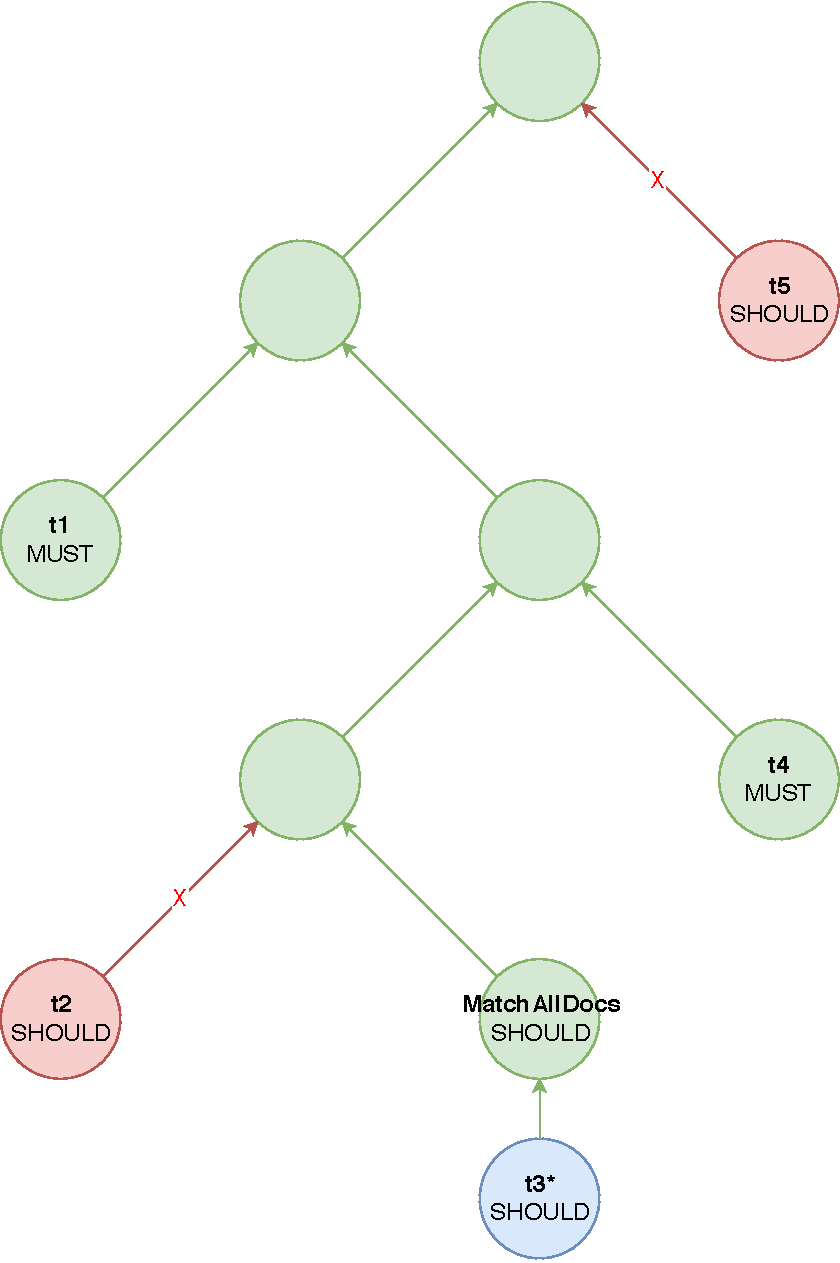
\includegraphics[width=80mm]{../img/complex_query.pdf}
    \caption{Grouping queries example tree representation}
    \label{group_tree}
\end{figure}

\subsection{Dealing with Fuzzy Factor}
\label{fuzzy}
It is possible to specify a fuzzy factor for the queries which indicates how well should the query match the documents.

\subsubsection{Fuzzy Search}
Lucene supports fuzzy searches which are based on the Levenshtein Distance
\footnote{\url{https://en.wikipedia.org/wiki/Levenshtein_distance}} algorithm. This option can be specified by typing
$\sim$ after the searched term and followed by the value of the fuzzy factor. However, it can only be specified for the
single term query. The Suggester supports this option. By writing the $\sim$ with the fuzzy factor after the term the
suggester will suggest the terms which satisfy this condition.

\subsubsection{Proximity Search}
Proximity search is a phrase query with a specified fuzzy value. The fuzzy value represents the allowed edit distance of the
tokens of the phrase query. The implementation is very similar to \ref{suggest_phrase_query}. However, the suggestions
take the fuzzy factor into account and will contain terms that satisfy this condition.

\subsection{Dealing with Boost Factor}
Lucene supports term boosting by writing \textbf{\^} after the searched term and followed by the value of the boost factor.
The default boost factor is 1. It must be positive but can be less than 1. The boost factor specifies how the term is relevant
in regard to other terms. In the query \ref{boost} the term \textit{term1} is more relevant than the term \textit{term2}.

\begin{equation}
\label{boost}
term1\ \hat{}\ 3\ \&\&\ term2
\end{equation}

It might be possible for complex queries to take this information and boost those suggested terms that are in the same
document as boosted term. However, for now, the boost factor is ignored by the suggester.

\subsection{Promoting Suggestions Based on the Previous Searches}
The \textbf{reciprocal rank} of a query response is the multiplicative inverse of the rank of the first correct answer.
That means, if the first correct answer was on the third place then reciprocal rank would be $\frac{1}{3}$.

\textbf{Mean reciprocal rank}\footnote{\url{https://en.wikipedia.org/wiki/Mean\_reciprocal\_rank}}(MRR) is defined as
average of reciprocal ranks for a set of queries $Q$. Mathematically, it is defined as in \ref{mrr}.

\begin{equation}
\label{mrr}
MRR = \frac{1}{\vert Q \vert} \sum_{i=1}^{\vert Q \vert} reciprocalRank_i
\end{equation}

In \citep{Bar-yossef11context-sensitivequery} multiple approaches are presented to the suggestions based on previous
searches:
\begin{itemize}
    \item \textbf{Most popular completion} – wisdom of the crowds. For some prefix the suggester suggests the terms
    with the same prefix that were searched the most.
    \item \textbf{Nearest completion} – takes into account current context of the user that is typing the queries.
    The authors defined \textbf{logical search session} as an interactive process in which the user (re-)formulates queries
    while searching for documents satisfying a particular information need. It consists of a sequence of
    queries $q_1, . . . , q_t (t \geq 1)$ issued by the user. The \textbf{context} of a user input $x$, where $x$ is the prefix of
    some query $q_i$ in the session, is the sequence of queries $q_1, . . . , q_{i-1}$ preceding $q_i$.
    Authors also specified how to convert context to a vector which can be used to find the most similar query.
    This works for vector model based search engines. Lucene is a combination of vector and boolean model so the
    conversion could be applicable.

    \item \textbf{Hybrid completion} – if there is no or almost no context then \textit{nearest completion} cannot predict the
    suggestions. Therefore, \textit{hybrid completion} is a combination of \textit{most popular completion} and \textit{nearest completion}.
    The authors have shown in empirical study that \textit{hybrid completion} has better \textit{MRR} than
    \textit{most popular completion} on average.
\end{itemize}


\textbf{Chosen solution} – \textit{nearest completion} and thus \textit{hybrid completion} are very intriguing and could
improve the suggestions by a big margin. However, they would need to be adapted to Lucene and the implementation
might not be completely straightforward. Therefore, the basic implementation of suggester will only include the
\textit{most popular completion}. Implementation of the \textit{nearest completion} is a very promising canditate for
future extensions.

\subsubsection{Most Popular Completion – Simple Queries}

To implement most popular completion the score of the terms needs to be changed by some factor. For instance, if the term
$term1$ was searched for $i$ times then the score could be changed by a number $h(i)$ for some function $h: \mathbb{N} \mapsto \mathbb{N}$.
It is also possible to take into account how recent the searches were and if there is a multiple recent searches for some
term then increase its score by a higher value. For instance, this could arise in a situation if some error was found in
method $m()$ of some well known library, then multiple users will probably be searching for it in a small time interval.
However, the suggester will focus only on the basic implementation that considers only the term search count mainly because
its simplicity. The time factor is a possible extension to an existing solution.

It is needed to have a key-value store for storing the number of searches for the terms. This store should be persistent
so the data would not be lost after the restart of the application. Also this store should allow parallel access for
efficiency. There are multiple options how to achieve this functionality:
\begin{itemize}
    \item \textbf{Java Map} implementation with concurrent access, e.g. \textit{ConcurrentHashMap}. This map could be stored
    on the disk periodically to fulfil the persistency requirement. This solution has a few drawbacks:
    \begin{itemize}
        \item Loss of recent data after restart/crash.
        \item The data are held in memory. The size of the data is non-trivial, e.g.
        \textit{Linux kernel} dataset contained approximately $3.5 million$ terms for \textit{full} field.
    \end{itemize}

    \item \textbf{Redis}\footnote{\url{https://redis.io}} – in-memory data structure store, used as a database, cache
    and message broker. It has support for multiple languages and contains the needed commands (\textit{GET, INCR}).
    The major drawback is that Redis would have to be installed and run separately. Although some embedded Redis solutions
    exist, those are meant for testing purposes. Redis also has support for persistence:
    \begin{itemize}
        \item \textbf{RDB} persistence – performs point-in-time snapshots of the dataset at specified intervals.
        \item \textbf{AOF} persistence – logs every write operation received by the server, that will be played again
        at server startup, reconstructing the original dataset.
    \end{itemize}

    \item \textbf{Relational Database} – even though traditional databases satisfy most of the needs, they do not
    provide the sufficient speed performance.

    \item \textbf{Chronicle Map}\footnote{\url{https://chronicle.software/products/map/}} – provides a Java Map like
    interface and stores data off-heap. The data can be persistent by the use of memory mapped
    files\footnote{\url{https://en.wikipedia.org/wiki/Memory-mapped\_file}}. On Linux machines it takes an advantage
    of lazy page allocation so the memory and disk usage can be small if it contains only a few entries.
    Disadvantages are that some hints are needed for the data structure to perform efficiently:
    \begin{itemize}
        \item Number of entries – can be overestimated. However, the authors specify that it would be best to specify
        this number to the actual number of entries stored $\pm 10\%$. Even though it is possible to store more elements
        than specified, the performance of the data structure decreases marginally.
        \item Average key size – does not affect maximum key size.
    \end{itemize}
    Another disadvantage is that some Java options are needed for it to work with Java 9 and later releases.

    \item \textbf{MapDB}\footnote{\url{http://www.mapdb.org}} – similar to Chronicle Map but no hints are necessary.

    \item \textbf{LMDB for Java}\footnote{\url{https://github.com/lmdbjava/lmdbjava}} – Java mapping for
    LMDB\footnote{\url{https://symas.com/lmdb/}}. Major drawbacks:
    \begin{itemize}
        \item Low level API – keys and values need to be passed in byte buffers.
        \item Hints needed:
            \begin{itemize}
                \item Number of entries – can be overestimated.
                \item Maximum key size – must be the same as the maximum term size in Lucene which is 32767 bytes.
            \end{itemize}
        \item Some Java options needed for Java 9 and later.
    \end{itemize}
\end{itemize}

Benchmarks comparing MapDB, Chronicle Map, LMDB for Java and some other solutions performed by the LMDB for Java creators
can be found in \citep{lmdb}.

A benchmark for similar usage as in our case comparing MapDB, Chronicle Map and LMDB for Java can be seen on the graph \ref{comp_maps}.
The performed test consists of getting the integer value for every 20th term of \textit{English words} dataset.
The details on how the benchmark was performed and how it can be replicated can be found in \ref{benchmark_attachment}.

\begin{figure}[htbp]
    \centering
    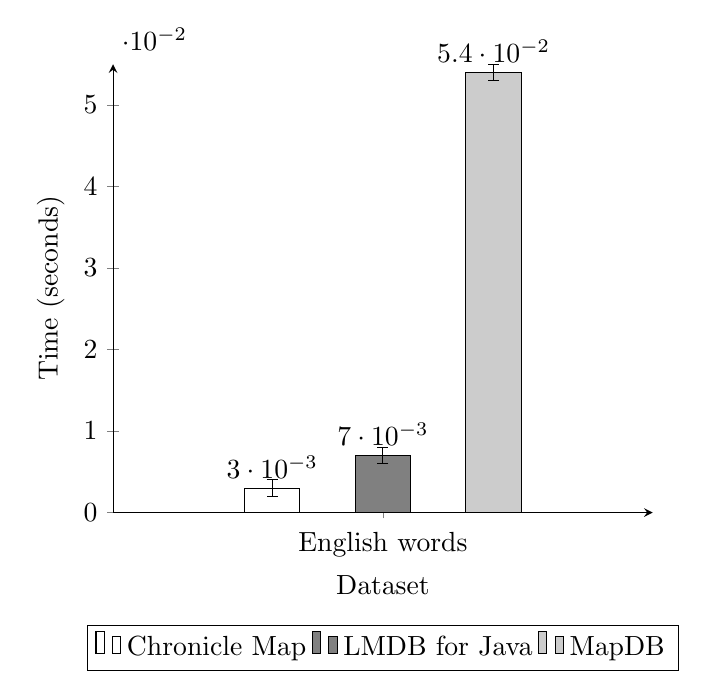
\begin{tikzpicture}
        \begin{axis}[
            ybar=20pt,
            bar width=20pt,
            xlabel={Dataset},
            ylabel={Time (seconds)},
            ymin=0,
            xtick=data,
            axis x line=bottom,
            axis y line=left,
            enlarge x limits=0.2,
            symbolic x coords={English words},
            xticklabel style={anchor=base,yshift=-\baselineskip},
            nodes near coords={\pgfmathprintnumber\pgfplotspointmeta},
            legend style={at={(0.5,-0.25)},anchor=north,legend columns=-1}
        ]
        \addplot[ybar, fill=white, error bars/.cd, y dir=both, y explicit] plot coordinates {
        (English words, 0.003) += (English words, 0.001) -= (English words, 0.001)
        };

        \addplot[ybar, fill=gray, error bars/.cd, y dir=both, y explicit] plot coordinates {
        (English words, 0.007) += (English words, 0.001) -= (English words, 0.001)
        };

        \addplot[ybar, fill=black!20, error bars/.cd, y dir=both, y explicit] plot coordinates {
        (English words, 0.054) += (English words, 0.001) -= (English words, 0.001)
        };

        \legend{Chronicle Map, LMDB for Java, MapDB}
        \end{axis}
    \end{tikzpicture}
    \caption{Comparison of lookup times for selected key-value stores}
    \label{comp_maps}
\end{figure}

Although MapDB provides the nicest high-level interface and there is no need to specify its size in advance,
its lookup speeds were lacking behind the other options.
In the end, Chronicle Map was chosen to serve as a key-value store because it had proven to have a very solid performance.

As mentioned in \ref{possible_implementations}, the best option for simple prefix queries is a WFST data structure.
Mainly because of its low memory footprint and fast lookups.
Every term has a score assigned based on its occurrence frequency as mentioned in \ref{prefix_scoring}. This score
can be computed at the start and does not change very often – only after performing reindex.

The best and easiest solution would be to change the term score in WFST directly. However, this is not possible because
Lucene's implementation of WFST is read-only. Let's examine possible modifications to WFST to allow changing the score of the
terms.
\begin{itemize}
    \item WFST is stored in a byte array (\textit{byte[]}) or multiple byte arrays to allow low memory footprint. The
    arc values are very often small because they only represent difference to the smallest term in the subtree. Lucene
    implementation leverages this and for small values less bytes need to be written. For instance, take an \textit{int}
    data type – it needs 4 bytes to be stored properly. However, in the WFST implementation it takes between 1 and 5 bytes.
    The smaller values need less space. Per byte, the highest order bit indicates whether the next byte is part of this
    number and the remaining 7 bits contain the actual value. Even though this allows for a very efficient memory requirements,
    the modifications are a problem. If we were to increase some value, then it might take more bytes than it actually has available.
    Therefore, part of the byte array would need to be shifted by 1 byte. This operation would prevent parallel access.
    One solution might be that there would be another array where the content would be copied and then the references
    would be swapped. However, this does not allow parallel modifications.
    Another solution is to discard the variable length of the values and allocate a constant size for them,
    e.g. 4 bytes for \textit{int}. This however increases the memory footprint as can be seen on \ref{enc_comp}.

    \begin{figure}[htbp]
        \centering
        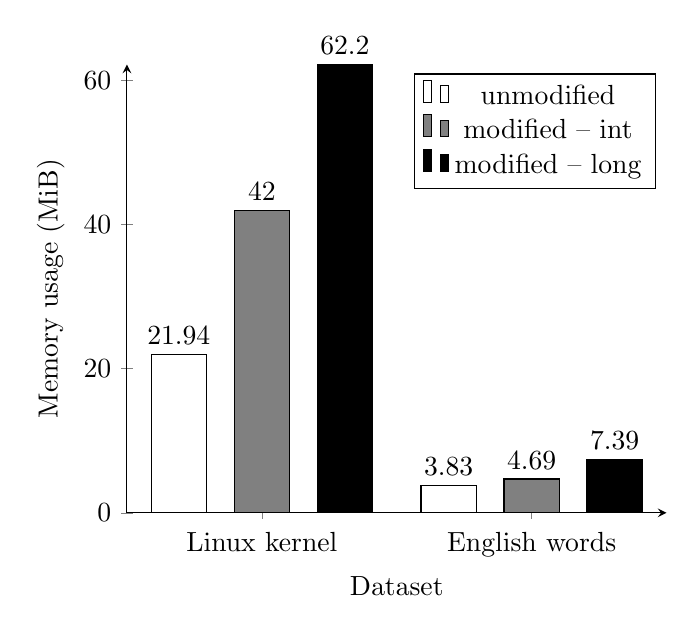
\begin{tikzpicture}
            \begin{axis}[
                ybar=10pt,
                bar width=20pt,
                xlabel={Dataset},
                ylabel={Memory usage (MiB)},
                ymin=0,
                xtick=data,
                axis x line=bottom,
                axis y line=left,
                enlarge x limits=0.5,
                symbolic x coords={Linux kernel, English words},
                xticklabel style={anchor=base,yshift=-\baselineskip},
                nodes near coords={\pgfmathprintnumber\pgfplotspointmeta}
            ]

            \addplot[ybar, fill=white, error bars/.cd, y dir=both, y explicit] plot coordinates {
            (English words, 3.8268890381)
            (Linux kernel, 21.9446716309)
            };

            \addplot[ybar, fill=gray, error bars/.cd, y dir=both, y explicit] plot coordinates {
            (English words, 4.6938095093)
            (Linux kernel, 41.9976768494)
            };

            \addplot[ybar, fill=black, error bars/.cd, y dir=both, y explicit] plot coordinates {
            (English words, 7.3886260986)
            (Linux kernel, 62.2045021057)
            };

            \legend{unmodified, modified – int, modified – long}
            \end{axis}
        \end{tikzpicture}
        \caption{Comparison of memory usage when changing number encoding}
        \label{enc_comp}
    \end{figure}

    The memory usage increased by approximately $22\%$ for \textit{English words} dataset. However, it can be
    almost doubled as can be seen on \textit{Linux kernel} dataset where approximately $92\%$ size increase can be noted.
    The graph \ref{enc_comp} also shows the case when the encoding would use \textit{long} datatype. Although Lucene's \textit{Lookup}
    interface specificies \textit{long} datatype, WFST implementation supports only \textit{int} so far.

    \item Lucene's WFST implementation does not know the notion of nodes but the data are stored only in arcs. Arcs that
    start in the root node might be stored in memory directly and therefore are not encoded in byte array since these
    arcs are acessed very often
    and the decoding from byte array has an impact on the data structure lookup performance. Although this is not a big issue,
    the modifications would need to take this into account and add checks for this case.

    \item In some cases (e.g. the depth of an arc is less than a constant or there is more arcs from one node than
    another constant) the arcs
    might not be encoded as efficiently as possible but rather take a constant size. This then allows to do a binary
    search of arcs rather than going over them sequentially. Thus, increasing the speed of the lookup.

    \item As explained in \ref{FST}, scores of the terms are inverted (\ref{invert_score}) so by increasing score of some term
    we are actually decreasing its weight in WFST. Sum of arc values on the path to a term is the weight of the term (plus the final output modifier).
    However, the arc value tries to represent the lowest weight of the term in its subtree. And by decreasing this weight
    it could be necessary to update the whole WFST data structure. For instance, let's suppose that we have WFST as in \ref{wfst_example}
    and that the weight of the term $CAR$ will change to value $2$. The changes can be seen on the \ref{wfst_modified} in red color.

    \begin{figure}[htbp]
    \centering
    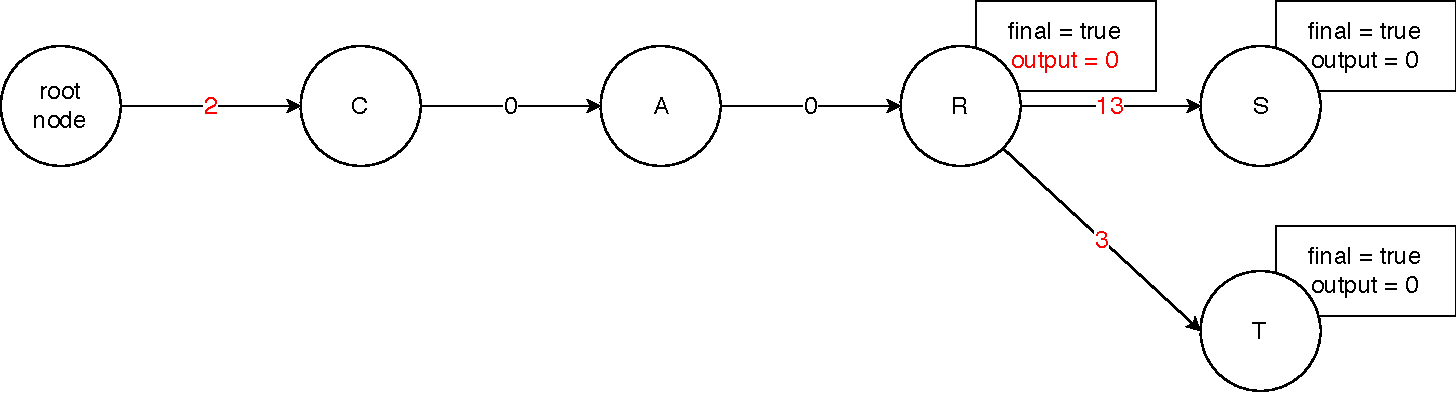
\includegraphics[width=145mm]{../img/wfst_modified.pdf}
    \caption{WFST modifications}
    \label{wfst_modified}
    \end{figure}

\end{itemize}

As a consequence of these observations, it was decided that modifying the WFST to allow changing scores could be a difficult
endeavour. Therefore, the remaining option was to rebuild WFSTs per some time interval. The most negative impact is that the
suggestions for simple queries will not take the other searches into account immediately but only after some non-trivial time period.

This time period should be configurable. There are a few options from which to choose:
\begin{itemize}
    \item \textbf{Period} – specified in some time unit. For instance, data should be rebuilt every hour. This solution
    is easy to implement. The period could start ticking at the last rebuilt. The main drawback is that there is no way
    how to specify the exact time.
    \item \textbf{Exact time} – is a good option when it is known when system load will be small (e.g. during the night).
    \item \textbf{Cron format}\footnote{\url{https://en.wikipedia.org/wiki/Cron}} – \label{cron} cron is a job scheduler for Unix
    operating system. When and which jobs should be run is specified in the special file called \textit{cron table}. The problem
    is that the Java does not have native support for processing this format and some library must be used, the most notable are:
    \begin{itemize}
        \item cron4j\footnote{\url{http://www.sauronsoftware.it/projects/cron4j/}} – simple library which allows to
        create simple scheduler with specified cron format and
        \textit{Runnable}\footnote{\url{https://docs.oracle.com/javase/10/docs/api/java/lang/Runnable.html}} that is to be performed.
        The provided interface is clean and to the point. However, at the time of writing, the library is no longer maintained and
        was not updated in 5 years.
        \item cron-utils\footnote{\url{https://github.com/jmrozanec/cron-utils}} - a small library for parsing and
        converting various cron formats. It also provides a feature which allows to compute the time to the next execution
        based on the cron format.
        \item quartz\footnote{\url{http://www.quartz-scheduler.org}} – is an enterprise job scheduler library which
        allows to create truly complex jobs.
    \end{itemize}
\end{itemize}

\textbf{Chosen solution} – it was desired to allow the administrators the most freedom. For that, the cron format was
deemed the best option. It was a hard choice to pick between the mentioned libraries. In the end, \textit{cron4j} was ruled out
because of its oldness and the \textit{quartz} because of its complexity. \textit{cron-utils} can be quite easily combined with
\textit{ScheduledExecutorService}\footnote{\url{https://docs.oracle.com/javase/10/docs/api/java/util/concurrent/ScheduledExecutorService.html}}
to create the needed functionality.

\subsubsection{Most Popular Completion – Complex Queries}
\label{previous_searches}
There are multiple possible approaches how to enhance the suggester with the use of complex queries:
\begin{itemize}
    \item Different term boosting – boost terms based on their popularity but also take into account other
    query parts. For example, if the search would be restricted to Java file types then the suggester could
    only boost terms which were searched for when this condition held true.
    \item Suggest the whole complex query – if the starts to write a part of a complex query then it could be recognized
    by the suggester which could suggest this already known query. However, this might not be user friendly since there
    are multiple search fields which content would have to modified. Or the whole query would need to be written by the
    use of field specifiers which might make the query badly readable.
\end{itemize}

Possible implementation of both suggested approaches would require additional data structures and could slow down the
suggester. For now, they are deemed only as a possible extension.

As a result, the complex query is only dismantled into simple term queries which are used to update the popularity term counts.

\subsubsection{Increasing Search Counts for Specific Terms}
Administrators might already have some search data stored. These data could be used to initialize or update the
popularity term counts.

There are 2 possible approaches how to do this:
\begin{itemize}
    \item By processing HTTP search request URLs:
        \begin{itemize}
            \item Target endpoint:
            \begin{itemize}
                \item Request method: POST
                \item Endpoint: /suggest/add
                \item Media type: application/json
            \end{itemize}
            \item Example data:
\begin{code}
["http://demo.opengrok.org/search?project=opengrok\&q=test"]
\end{code}
        \end{itemize}
    \item By processing JSON data:
        \begin{itemize}
            \item Target endpoint:
            \begin{itemize}
                \item Request method: POST
                \item Endpoint: /suggest/add
                \item Media type: application/json
            \end{itemize}
            \item Example data:
\begin{code}
[{"project": "opengrok", "field": "full", "token": "test", "increment": 1}]
\end{code}
        \end{itemize}
\end{itemize}

\subsubsection{User Specific Suggestions}
The Suggester might be further extended to provide suggestions based on the user specific previous searches. Google does
something similar as is highlighted by the number $1$ in the Figure \ref{google_previous}. Since authorization is optional
in OpenGrok, it would be best to store the previous search data in browser
cookies\footnote{\url{https://en.wikipedia.org/wiki/HTTP_cookie}}. This data could then be processed and
prepended to the returned suggestions from the Suggester.
However, the implementation of this feature is considered as a possible extension.

\begin{figure}[htbp]
    \centering
    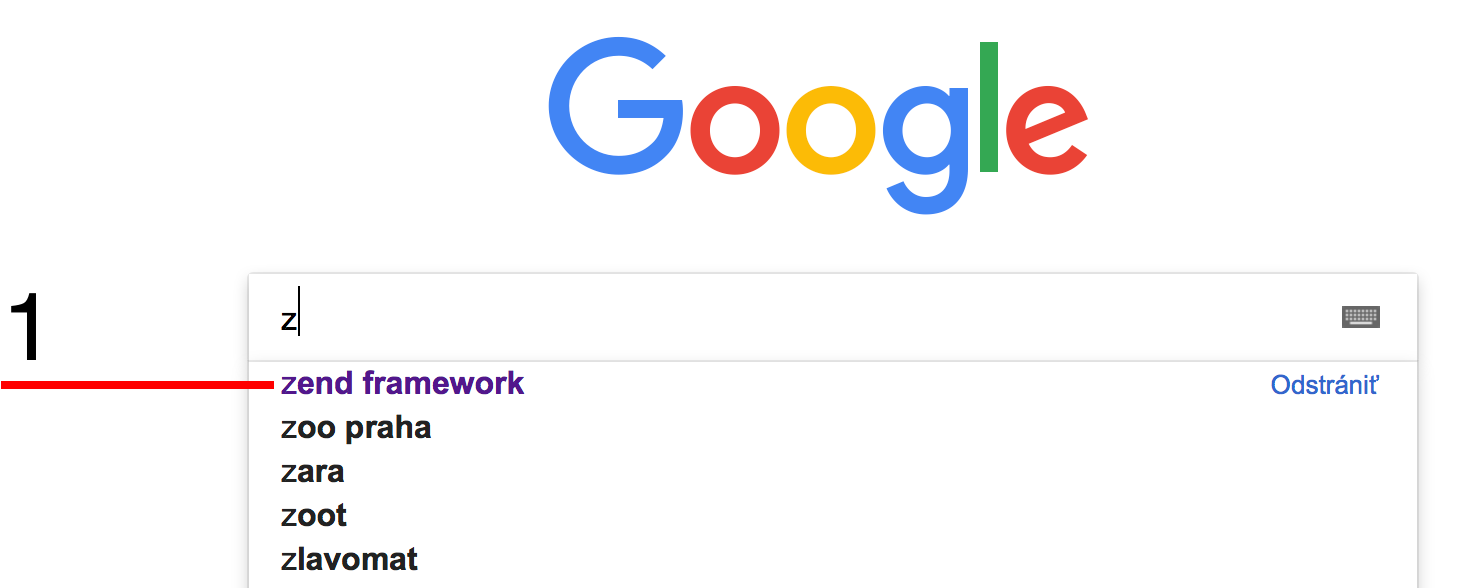
\includegraphics[width=100mm]{../img/google_previous.png}
    \caption{Suggestions based on the user specific previous searches by Google}
    \label{google_previous}
\end{figure}

\subsection{Do not Suggest the Same Term Already in the Query}
It can easily happen that user selects the first suggested item for some prefix $p$. If the user were to write the same
prefix again then the suggester should not offer the term that is already in the query.

For instance, imagine that the search field contains value $c\vert$ ($\vert$ signifies the input caret). The suggester
suggests values \textit{cat, color}. If the user chooses \textit{cat} and again types \textit{c} then the result
query has format $cat\ c\vert$. In this case the suggester should not suggest the \textit{cat} value but only the \textit{color}
value.

\subsection{Authorization}
As specified in \ref{opengrok_overview}, the OpenGrok allows the administrators to specify to which projects have the users
access. Therefore, suggester must not allow unauthorized users to see suggestions because it would be considered as a security issue.

\subsection{Configuration}
\label{suggester_config}
As mentioned in \ref{opengrok_configuration}, OpenGrok can be configured using a configuration file.
Suggester should be also configurable to allow the users to specify how they want the suggester to perform.
Instead of creating its own separate way how to handle configuration, it will depend on the already existing solution in
OpenGrok. The main advantage is that the users are already familiar with how the configuration works. Configurable
properties of the suggester:
\begin{itemize}
    \item \textbf{Enabled} – specifies if the suggester is enabled. Some users might not want the suggester functionality.
    Default value: \textit{true}.
    \item \textbf{Maximum results} – specifies how many results suggester should return at maximum. The lesser number may
    increase the suggester performance. Default value: \textit{10}.
    \item \textbf{Minimum characters} – specifies minimum number of characters that are needed for suggester to start looking
    for suggestions. The more characters means less possible candidates. Can significantly improve performance of the
    suggester. Default value: \textit{0}.
    \item \textbf{Allowed projects} – specifies set of projects for which the suggester should be enabled. Default value: \textit{all}.
    \item \textbf{Maximum projects} – specifies how many maximum projects can be selected at the same time and the suggestions will work.
    Default value: \textit{unlimited}.
    \item \textbf{Allowed fields} – specifies the fields for which the suggester should be enabled. For instance, it might be
    desired that the suggestions should only work for \textit{full} field. OpenGrok uses some fields to store
    private data and it is not desired to create suggester data structures for those fields. Therefore, only the main
    search fields are specified by default.
    Default value: \textit{full, defs, refs, path, hist, type}.
    \item \textbf{Allow complex queries} – specifies if the suggester should support complex queries. If set to
    \textit{false} then only simple prefix lookups by using the WFST data structure will be performed. Default value:
    \textit{true}.
    \item \textbf{Allow most popular} – specifies if the most popular completion should be enabled.
    If set to \textit{false} then it slightly increases the performance and there is no need for WFST rebuilds. Default value: \textit{true}.
    \item \textbf{Show scores} – specifies if the scores should be displayed next to the suggestions.
    Default value: \textit{false}.
    \item \textbf{Show projects} – specifies if the suggestions should show in which project the term was found.
    If there are multiple projects then showing all the names is not feasible; therefore, only the number of projects will be shown.
    Default value: \textit{false}.
    \item \textbf{Show time} – specifies if the time it took the suggester to find the suggestions should be displayed.
    Default value: \textit{false}.
    \item \textbf{Rebuild cron config} – specifies how often should the suggester rebuild the WFST data structures.
    The value must be in Unix cron format, decision is described in \ref{cron}.  Default value: \textit{0 0 * * *} (every day at midnight).
    \item \textbf{Build Termination Time in Seconds} – specifies after how much time the suggester should kill the
    threads that build the suggester data structures. Slow machines should specify more time. This option is mainly here
    to prevent the suggester to hang in the initialization. Default value: \textit{1800} (30 minutes).
\end{itemize}

\subsection{Tolerating Errors}
Although it is possible to use fuzzy factor as specified in \ref{fuzzy}, the Suggester is not error tolerant.
This could be a good extension to the prefix queries \ref{prefix_query}.
For instance, if the user types prefix \textit{sh} even though
the index contains the term \textit{schwarz}, it won't be among the suggestions. This might prove very useful if the
user made a typing error or is not sure about the spelling of the term.

\citep{Chaudhuri09extendingautocompletion} studies the possibility of tolerating errors for prefix autocompletion.
Authors defined prefix $p$ as a \textit{k-prefix} of string $s$ if there is some extension of $p$ that is within edit
distance $k$ of $s$. $s$ is called a \textit{k-extension}. Then, for some prefix it is possible to consider its
k-extensions up to some constant $k$. Authors presented Trie and Q-gram based algorithms. However, this would need
another data structures and does not work for other types of queries. Therefore, it is considered as a possible extension.
